\chapter{Richiami di Elettronica} \label{chapter: RichiamiElettronica}

%----------------------------------------------------------------------%
%                            Prima sezione                             %
%----------------------------------------------------------------------%
% Nella prima sezione faccio una rapida introduzione ed un breve       %
% ripasso di concetti basilari del campo dell'elettronica: per fornire %
% un esempio pratico effettuo l'analisi del circuito RC, comoda anche  %
% per comprendere meglio gli effetti di feedback che portano ad una    %
% distruzione della colonna di plasma.                                 %
%----------------------------------------------------------------------%

\section{Introduzione}

In questo capitolo sono presenti alcuni rudimenti di elettronica che consentono di comprendere meglio il funzionamento del
setup sperimentale che viene utilizzato in laboratorio. Iniziamo quindi ricordando la definizione di corrente elettrica, che
si esprime matematicamente come la derivata della carica elettrica rispetto al tempo:
\begin{equation}
    I\,=\,\frac{dQ}{dt}.
    \label{equation: current}
\end{equation}
I circuiti elettrici sono formati da elementi circuitali interconnessi tra di loro: un esempio ne sono i bipoli elettrici, 
che sono dispositivi a due terminali. Il più semplice bipolo lineare è la \textbf{resistenza}, le cui caratteristiche sono racchiuse
nella \textit{Legge di Ohm}:
\begin{equation}
    V\,=\,RI.
    \label{equation: OhmLaw}
\end{equation}
\begin{figure}[H]
    \centering
    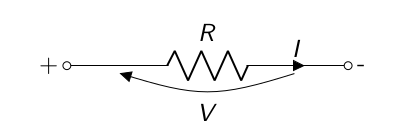
\includegraphics[width=0.5\textwidth]{Immagini/Resistenza.png}
    \caption{Rappresentazione schematica di una resistenza}
    \label{figure: resistenza}
\end{figure}
Un punto comune a due o più bipoli è detto nodo: i bipoli si possono disporre in modo tale da formare dei percorsi chiusi,
detti maglie. I concetti di nodo e maglia consentono di semplificare l'analisi di circuiti complessi per mezzo delle 
\textit{Leggi di Kirchoff}. La \textit{KVL (Kirchoff Voltage Law)} afferma che lungo una qualsiasi maglia di un circuito
la somma algebrica di tutte le tensioni è pari a zero:
\begin{equation}
    \sum_{k\,\in\,maglia}V_k\,=\,0,
    \label{equation: KVL}
\end{equation}
dove si considerano positive le tensioni concordi con il verso di percorrenza della maglia e negative le tensioni discordi.
La \textit{KCL (Kirchoff Current Law)} riguarda invece le correnti ed evidenzia come in un qualsiasi nodo di un circuito
la somma algebrica di tutte le correnti è identicamente nulla
\begin{equation}
    \sum_{k\,\in\,maglia}I_k\,=\,0,
    \label{equation: KCL}
\end{equation}
dove sono positive le $I_k$ entranti nel nodo, mentre negative quelle uscenti.
\begin{figure}[H]
    \centering
    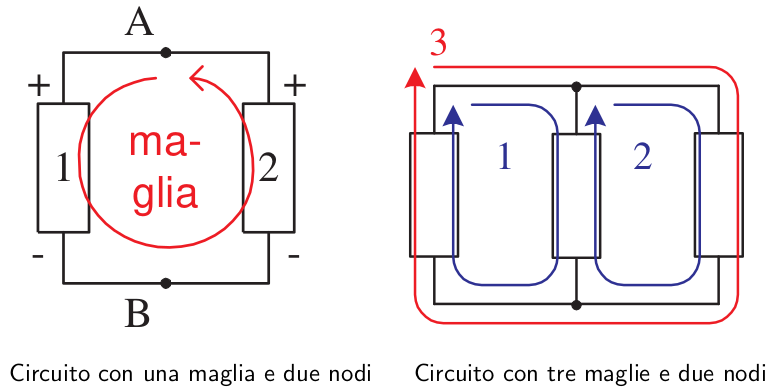
\includegraphics[width=0.9\textwidth]{Immagini/EsempioMaglie.png}
    \caption{Esempi di maglie in un circuito}
    \label{figure: KirchoffLaws}
\end{figure}
Un altro esempio di bipolo è il \textbf{condensatore}, che è un elemento circuitale costituito da due superfici metalliche 
parallele separate da un isolante. Le armature metalliche possono immagazzinare della carica, in quantità proporzionale alla
tensione applicata
\begin{equation}
    q(t)\,=\,Cv(t),
    \label{equation: capacità}
\end{equation}
dove con $C$ si indica la capacità del condensatore, misurata in farad (F).
\begin{figure}[H]
    \centering
    \includegraphics[width=0.5\textwidth]{Immagini/Capacità.png}
    \caption{Rappresentazione schematica di un condensatore}
    \label{figure: resistenza}
\end{figure}
L'ultimo esempio di bipolo a cui siamo interessati è l'\textbf{induttore}, che è costituito da un filo di materiale
conduttore percorso da corrente (solenoide).
All'interno dell'avvolgimento si ha un flusso di campo magnetico $\Phi$ che è proporzionale alla corrente che percorre il
filo
\begin{equation}
    \Phi(t)\,=\,Li(t),
    \label{equation: induttanza}
\end{equation}
dove $L$ è l'induttanza dell'induttore e si misura in henry (H).
\begin{figure}[H]
    \centering
    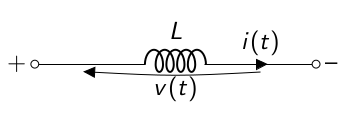
\includegraphics[width=0.5\textwidth]{Immagini/Induttanza.png}
    \caption{Rappresentazione schematica di un induttore}
    \label{figure: induttanza}
\end{figure}

\subsection{Circuito RC}

Il circuito RC è un circuito del primo ordine, ossia è caratterizzato da un'equazione differenziale del primo ordine. 
\begin{figure}[H]
    \centering
    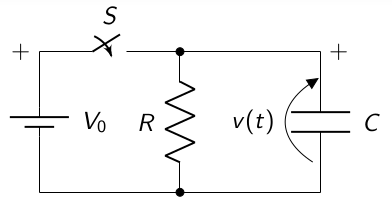
\includegraphics[width=0.65\textwidth]{Immagini/CircuitoRC.png}
    \caption{Rappresentazione schematica di un circuito RC}
    \label{figure: CircuitoRC}
\end{figure}
Gli elementi circuitali presenti sono tre:
\begin{list}{\textbf{-}}{\setlength{\itemsep}{0cm}}
    \item un interruttore ideale $S$ che si comporta come un circuito aperto quando è spento e come un cortocircuito quando
    è acceso
    \item una resistenza $R$
    \item un condensatore $C$
\end{list}
Quando l'interruttore è acceso si assiste ad una carica del condensatore: la differenza di potenziale $v(t)$ è pari a quella
dovuta al generatore di tensione $V_0$. Mediante le semplici relazioni \eqref{equation: OhmLaw} e \eqref{equation: capacità}
introdotte in precedenza è possibile ricavare i valori di corrente nel resistore e di carica immagazzinata nel condensatore.
Supponiamo ora di aprire l'interruttore scollegando di fatto il generatore di tensione: per risolvere il circuito occorre
lavorare con le leggi di Kirchoff. In particolare notiamo che
\begin{equation}
    i_R\left(t\right)\,+\,i_C\left(t\right)\,=\,0,
    \label{equation: KCL_circuitoRC}
\end{equation}
dove gli indici si riferiscono ai due elementi circuitali presente nell'unica maglia del circuito RC una volta aperto.
La relazione \eqref{equation: KCL_circuitoRC} è un'equazione differenziale del primo ordine per la differenza di potenziale
ai capi del condensatore, poichè effettuando le opportune sostituizioni è possibile mostrare come 
\begin{equation}
    \frac{v\left(t\right)}{R}\,+\,C\frac{dv\left(t\right)}{dt}=\,0.
    \label{equation: EqDiff_circuitoRC}
\end{equation}
Notiamo che la soluzione di \eqref{equation: EqDiff_circuitoRC} sia un esponenziale reale, che imponendo la condizione iniziale
di potenziale al tempo dello spegnimento dell'interruttore pari a $V_0$ risulta essere
\begin{equation}
    v\left(t\right)\,=\,V_0\exp{\left(-\frac{t}{RC}\right)}.
    \label{equation: solEqDiff_circuitoRC}
\end{equation}


%----------------------------------------------------------------------%
%                           Seconda sezione                            %
%----------------------------------------------------------------------%
% Nella seconda sezione faccio un rapido ripasso sulla trasformata di  %
% Fourier in modo tale da introdurre come lo studio delle equazioni    %
% differenziali nel dominio delle frequenze si traduca nel trovare le  %
% soluzioni di equazioni algebriche. Fornisco un esempio di questo     %
% processo con la risoluzione del circuito RC passa basso              %
%----------------------------------------------------------------------%


\section{Dominio delle frequenze}

Lavorare nello spazio delle frequenze per risolvere i circuiti elettrici è vantaggioso, perchè si assiste ad una notevole
semplificazione dei calcoli da compiere: le equazioni differenziali presenti nel dominio del tempo che governano il comportamento
dei circuiti RLC (resistori, induttori, condensatori) diventano delle relazioni algebriche. Nel dominio delle frequenze gli
elementi circuitali che abbiamo precedentemente introdotto sono rappresentati in termini di impedenza o ammettenza, che si
comportano come resistenze in un'analisi algebrica: questo rende più immediata l'analisi dei circuiti. Nel dominio delle
frequenze è anche possibile effettuare un'analisi della risposta in frequenza, cruciale per la progettazione di filtri.

\subsection{Trasformata di Fourier}

Un segnale è periodico quando si ripete identicamente dopo un intervallo di tempo $T$, detto periodo: l'inverso del periodo
è la frequenza e viene solitamente indicata con la lettera $f$. Ogni \textbf{segnale periodico} $x(t)$ con periodo $T\,=\,1/f_0$ può+
essere espresso come \textbf{serie di Fourier}
\begin{equation}
    x\left(t\right)\,=\,\frac{1}{2}a_0\,+\,\sum_{k\,=\,1}^{\infty}\left[a_k\cos{\left(2k\pi f_0t\right)}\,+\,b_k\sin{\left(2k\pi f_0t\right)}\right],
    \label{equation: SerieFourier}
\end{equation}
dove $a_k$ e $b_k$ sono detti coefficienti di Fourier e si ottengono mediante integrazione su un periodo del segnale di partenza
che si vuole ricostruire
\begin{equation}
    a_k\,=\,\frac{2}{T}\int_{-\frac{T}{2}}^{\frac{T}{2}} x\left(t\right)\cos{\left(2k\pi f_0t\right)}dt,
    \label{equation: a_coeffFourier}
\end{equation}
\begin{equation}
    b_k\,=\,\frac{2}{T}\int_{-\frac{T}{2}}^{\frac{T}{2}} x\left(t\right)\sin{\left(2k\pi f_0t\right)}dt.
    \label{equation: b_coeffFourier}
\end{equation}
Lavorando con le \textit{formule di Eulero} per il seno ed il coseno è possibile scrivere la serie di Fourier in forma complessa:
\begin{equation}
    x\left(t\right)\,=\,\sum_{k\,=\,-\infty}^{\infty}c_k \exp{\left(j2k\pi f_0t\right)},
    \label{equation: Compl_SerieFourier}
\end{equation}
dove $c_k$ sono dei coefficienti complessi tali per cui
\begin{equation}
    c_k\,=\,c_{-k}^*\,=\,\frac{a_k\,-\,jb_k}{2}\,=\,\frac{1}{T}\int_{-\frac{T}{2}}^{\frac{T}{2}} x(t)\exp{\left(-j2k\pi f_0t\right)} dt
    \label{equation: complex_coeff}
\end{equation}
Un segnale non periodico può essere considerato come un segnale periodico caratterizzato da un periodo tendente ad infinito
(e di conseguenza una frequenza caratteristica tendente a zero): in questo caso l'analisi di Fourier prevede il passaggio
dalla sommatoria all'integrale. Si identifica con il nome \textbf{Trasformata di Fourier} di un segnale $x\left(t\right)$ la
seguente quantità:
\begin{equation}
    X\left(f\right)\,=\,\mathcal{F}\left(x\left(t\right)\right)\,=\,\int_{-\infty}^{\infty}x\left(t\right)\exp\left(-j2\pi ft\right) dt.
    \label{equation: FourierTransform}
\end{equation}
L'anti-trasformata consente di effettuare il passaggio inverso, ossia da dominio delle frequenze al dominio del tempo e si
differenzia dalla trasformata per il segno dell'esponente (che è quindi positivo nel caso di $\mathcal{F^{-1}}$) e per il
fatto che l'integrazione viene effettuata sulle frequenze.

La trasformata di Fourier consente di studiare le equazioni differenziali che risolvono i circuiti nello spazio delle frequenze, 
dove figurano come equazioni algebriche: questo è possibile poichè valgono le seguenti relazioni
\begin{equation}
    \frac{dx\left(t\right)}{dt}\,\longleftrightarrow\,j2\pi fX\left(f\right),
    \label{equation: fourierDerivata}
\end{equation}
\begin{equation}
    \int x\left(t\right)dt\,\longleftrightarrow\,\frac{1}{j2\pi f}X\left(f\right).
    \label{equation: fourierIntegrale}
\end{equation}

\subsection{Impedenza}

Passando dal dominio del tempo al dominio della frequenza per mezzo della trasformata di Fourier, notiamo che vale per tutti
e tre gli elementi circuitali una relazione lineare fra intensità di corrente e differenza di potenziale: è infatti possibile
scrivere che
\begin{equation}
    V\left(f\right)\,=\,Z\left(f\right)I\left(f\right),
    \label{equation: impedenza}
\end{equation}
dove $Z\left(f\right)$ è l'impedenza, una quantità che si misura in ohm e che per elementi circuitali in serie o in parallelo
si compone analogamente ad una resistenza.
\begin{figure}[H]
    \centering
    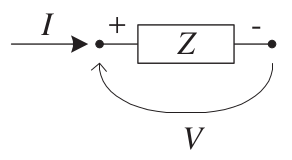
\includegraphics[width=0.35\textwidth]{Immagini/Impedenza.png}
    \caption{Rappresentazione schematica di un'impedenza}
    \label{figure: Impedenza}
\end{figure}
Nei casi dei tre bipoli presi in considerazione le impedenze sono differenti fra loro, infatti si ha che nel caso di:
\begin{equation}
    \text{un resistore} \longleftrightarrow Z\left(f\right)\,=\,R
    \label{equation: impedenzaR}
\end{equation}
\begin{equation}
    \text{un'induttanza} \longleftrightarrow Z\left(f\right)\,=\,j2\pi fL
    \label{equation: impedenzaL}
\end{equation}
\begin{equation}
    \text{un condensatore} \longleftrightarrow Z\left(f\right)\,=\,\frac{1}{j2\pi fL}
    \label{equation: impedenzaC}
\end{equation}
L'impedenza $Z$ è una grandezza complessa: la sua parte reale è la resistenza $R$, mentre la parte immaginaria prende il
nome di reattanza $X$.

\subsection{Risposta in frequenza}

La \textbf{risposta in frequenza} $H\left(f\right)$ di un circuito è definita come il rapporto fra i segnali di uscita e di
ingresso nel dominio della frequenza, ossia come
\begin{equation}
    H\left(f\right)\,=\,\frac{X_o(f)}{X_i(f)},
    \label{equation: rispostaFrequenza}
\end{equation}
dove con $X_i\left(f\right)$ e $X_o\left(f\right)$ sono indicate le trasformate di Fourier dei segnali in ingesso ed in uscita 
da un circuito. Solitamente la risposta in frequenza (che è una quantità complessa) viene espressa in termini di modulo 
$|H\left(f\right)|$ e fase $\angle H\left(f\right)$, ossia in coordinate polari nel piano complesso: i diagrammi di Nyquist 
sono la rappresentazione della traiettoria di $H\left(f\right)$ nel piano complesso.
\begin{figure}[H]
    \centering
    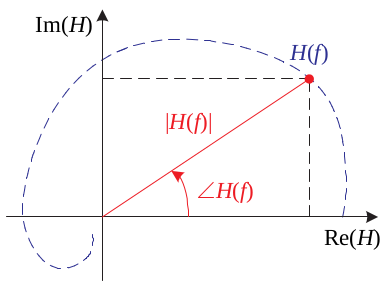
\includegraphics[width=0.35\textwidth]{Immagini/DiagrammaNyquist.png}
    \caption{Esempio di diagramma di Nyquist}
    \label{figure: Impedenza}
\end{figure}
Notiamo che se l'ingresso è unitario, l'uscita coinciderà con la risposta in frequenza: dato che $X_i\left(f\right)\,=\,1$ se
se $x_i\left(t\right)\,=\,\delta\left(t\right)$, concludiamo che $H\left(f\right)$ è la trasformata di Fourier della risposta
ad un impulso (risposta impulsiva).

\subsubsection{Diagrammi di Bode}

Per rappresentare graficamente $H\left(f\right)$ si utilizzano i \textbf{diagrammi di Bode}. Tali grafici sono di due tipi:
\begin{list}{\textbf{-}}{\setlength{\itemsep}{0cm}}
    \item per le \textbf{ampiezze}, dove in ascissa si riporta la frequenza $f$ in scala logaritmica, mentre in ordinata il
          modulo del guadagno in decibel.
    \item per la \textbf{fase}, che è analogo al precedente per quanto riguarda le scisse, mentre in ordinata riporta lo 
          sfasamento.
\end{list}

\subsection{Circuito RC passa-basso}

\begin{figure}[H]
    \centering
    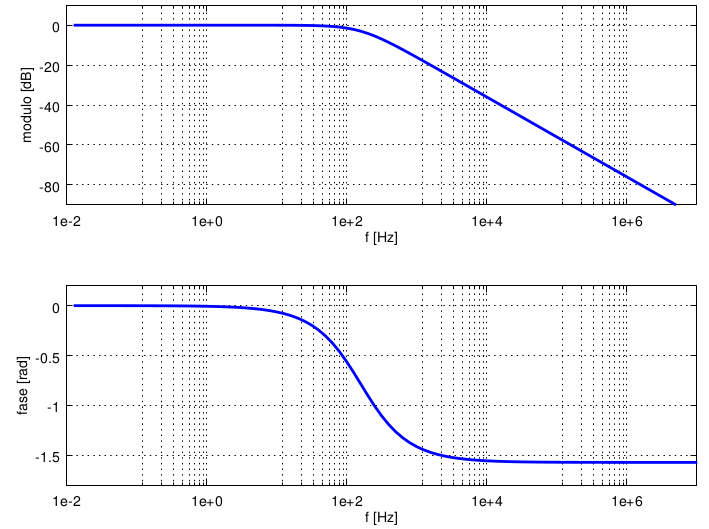
\includegraphics[width=0.75\textwidth]{Immagini/DiagrammiBodePassaBasso.png}
    \caption{Diagrammi di Bode del circuito $RC$ passa-basso.}
    \label{figure: Impedenza}
\end{figure}
